\chapter{Energy Storage: The Capacitor and Intermittent Operation}
\label{ch:capacitor}

\begin{defbox}[In this chapter you will learn]
\begin{itemize}
 \item the circuit model of a harvester feeding a capacitor through a series resistor, with leakage and a load;
 \item how to solve it: time constants, steady state, charge time, sustainable current;
 \item how Amber discretises the model with a 1\,ms step and why the discretisation is accurate;
 \item why a node needs \emph{two} voltage thresholds (hysteresis), how big an ``energy window'' they create, and the \emph{duty-cycle theorem} $D=P_{\mathrm{in}}/P_{\mathrm{active}}$;
 \item the \emph{energy-accounting} subtlety in the simulator's charge-while-active step, with a measured size of its effect.
\end{itemize}
\end{defbox}

\section{Why a capacitor?}

A harvesting node needs somewhere to \emph{accumulate} energy between its brief
bursts of activity. A rechargeable battery has high energy density but wears out,
leaks chemically and is costly; a \emph{capacitor} (or supercapacitor) stores less but
can be charged and discharged almost without limit, which suits devices intended to
live for a decade. Its great limitation is that its voltage is not constant:
\begin{equation}
 Q=CV,\qquad E=\tfrac12CV^{2},\qquad i=C\frac{\mathrm{d}V}{\mathrm{d}t}.
\label{eq:cap}
\end{equation}
Draining a capacitor lowers its voltage, and electronics need a minimum voltage.
The \emph{usable} energy is therefore only that between two voltages, a point
that drives the threshold logic of Section~\ref{sec:hysteresis}.

\section{The circuit}
\label{sec:circuit}

Amber's capacitor sees the circuit of Figure~\ref{fig:rccircuit}: the harvester
as a source $\Vs$ behind a series resistance $\Rs$ (Section~\ref{sec:amberharvest}), the
capacitor $C$, a parallel \emph{leakage} resistance $\Rl$ that models
self-discharge, and a load that draws a current $I_L$ chosen by the node's
state.

\begin{figure}[t]
\centering
\begin{circuitikz}[american,scale=0.95,transform shape]
 \draw (0,0) to[V,invert,l=$V_{\mathrm{src}}$] (0,2.6) to[R,l=$R_{\mathrm{s}}$] (3.0,2.6) -- (4.4,2.6);
 \draw (4.4,2.6) to[C,l=$C$,v=$V$,*-*] (4.4,0) -- (0,0);
 \draw (4.4,2.6) -- (6.8,2.6) to[R,l=$R_{\mathrm{l}}$,*-*] (6.8,0) -- (4.4,0);
 \draw (6.8,2.6) -- (9.2,2.6) to[I,l=$I_L$,*-*] (9.2,0) -- (6.8,0);
 \node[lab,align=center,anchor=north] at (0,-0.1) {harvester\\(Ch.~\ref{ch:harvest})};
 \node[lab,align=center,anchor=north] at (6.8,-0.1) {leakage};
 \node[lab,align=center,anchor=north] at (9.2,-0.1) {node load\\(Ch.~\ref{ch:controller})};
\end{circuitikz}
\caption{Equivalent circuit of Amber's energy store. Typical demo values: $\Rs=\SI{5}{k\ohm}$, $\Rl=\SI{100}{k\ohm}$, $C=\SI{300}{\micro F}$ (\SI{200}{\micro F} in the SIC demo); the load current $I_L$ takes values \SIrange{0.14}{5}{mA} depending on the node's state.}
\label{fig:rccircuit}
\end{figure}

Kirchhoff's current law at the capacitor node gives the governing equation
\begin{equation}
 C\frac{\mathrm{d}V}{\mathrm{d}t}\;=\;\frac{\Vs-V}{\Rs}\;-\;\frac{V}{\Rl}\;-\;I_L.
\label{eq:ode}
\end{equation}

\section{Solving it}
\label{sec:ode}

For a constant $\Vs$ and $I_L$, Eq.~\eqref{eq:ode} is linear first order. Define
\begin{equation}
 \tau=(\Rs\parallel\Rl)\,C=\frac{\Rs\Rl}{\Rs+\Rl}\,C,\qquad
 V_\infty=\big(\Vs-I_L\Rs\big)\frac{\Rl}{\Rl+\Rs}.
\label{eq:tauvinf}
\end{equation}
Then
\begin{equation}
 V(t)=V_\infty+\big(V_0-V_\infty\big)\,\e^{-t/\tau}.
\label{eq:vsol}
\end{equation}
Look at what the pieces mean.

\paragraph{Time constants.}
With the demo's $\Rs=\SI{5}{k\ohm}$, $\Rl=\SI{100}{k\ohm}$, $C=\SI{300}{\micro F}$:
the charging constant is $\tau_c=\Rs C=\SI{1.5}{s}$, the leakage constant
$\tau_\ell=\Rl C=\SI{30}{s}$, and the effective constant
$\tau=\SI{1.43}{s}$ is dominated by charging.

\paragraph{Steady state.}
With no load ($I_L=0$) the capacitor settles at
$\Vs\,\Rl/(\Rl+\Rs)$: a \emph{voltage divider} between the series and
leakage resistances. With $\Rl/\Rs=20$ the final voltage is $95.2\%$ of $\Vs$; leakage steals about
$5\%$. If a load draws $I_L$, the steady voltage falls by $I_L\Rs\,\Rl/(\Rl+\Rs)$.
A node is \emph{energy-starved} if $V_\infty<\Vlow$ for its typical load: it can never
sustain operation.

\paragraph{Sustainable current.}
At voltage $V$ the harvester can supply a steady current $(\Vs-V)/\Rs$ and leakage takes
$V/\Rl$, so the \emph{sustainable} load is
\begin{equation}
 I_{\max}(V)=\frac{\Vs-V}{\Rs}-\frac{V}{\Rl}.
\end{equation}
At $V=\SI{1.5}{V}$, Node~0 ($\Vs=\SI{2.49}{V}$) can sustain $\SI{182}{\micro A}$, which
exceeds the $\SI{140}{\micro A}$ listening current: it could idle in the listening state indefinitely.
Node~1 ($\Vs=\SI{1.97}{V}$) can sustain only $\SI{79}{\micro A}$, so even
continuous listening would drain it; it \emph{must} duty-cycle. This one-line
calculation predicts a lot about who will be awake.

\paragraph{Time to reach a threshold.}
Solving Eq.~\eqref{eq:vsol} for $V(t)=V_{\mathrm{th}}$ starting at $V_0<V_{\mathrm{th}}<V_\infty$:
\begin{equation}
 t_{\mathrm{th}}=\tau\,\ln\frac{V_\infty-V_0}{V_\infty-V_{\mathrm{th}}}.
\label{eq:tth}
\end{equation}

\begin{example}[Activation times of the demo nodes]
From $V_0=0$ with $\Vhigh=\SI{1.7}{V}$ and no load:
\begin{center}
\small
\renewcommand{\arraystretch}{1.1}
\begin{tabular}{@{}lrrrr@{}}
\toprule
Node & $\Vs$ (V) & $V_\infty$ (V) & $t_{1.7\,\mathrm{V}}$ (s) & Remark\\
\midrule
Node 0, WPT, \SI{20}{m} & 2.486 & $2.37$ (clamped to $2.0$) & 1.81 & \\
Node 1, WPT, \SI{30}{m} & 1.971 & 1.88 & 3.37 & slower\\
Node 2, RF only & 0.662 & 0.63 & never & $V_\infty<\Vhigh$\\
Node 2, solar (mean) & 2.665 & 2.54 (clamped to $2.0$) & 1.58 & what the demo uses\\
\bottomrule
\end{tabular}
\end{center}
The measured activations in Figure~\ref{fig:sawtooth} ($\approx1.8$, $\approx3.4$ and
$\approx\SI{1.4}{s}$) agree; Node~2's slightly earlier activation reflects the trace's initial
values ($\approx\SI{2.7}{V}$ to $\SI{3.0}{V}$). A random start-up delay of up to $\SI{2}{s}$ (Chapter~\ref{ch:controller})
can postpone activation further.
\end{example}

\begin{figure}[t]
\centering
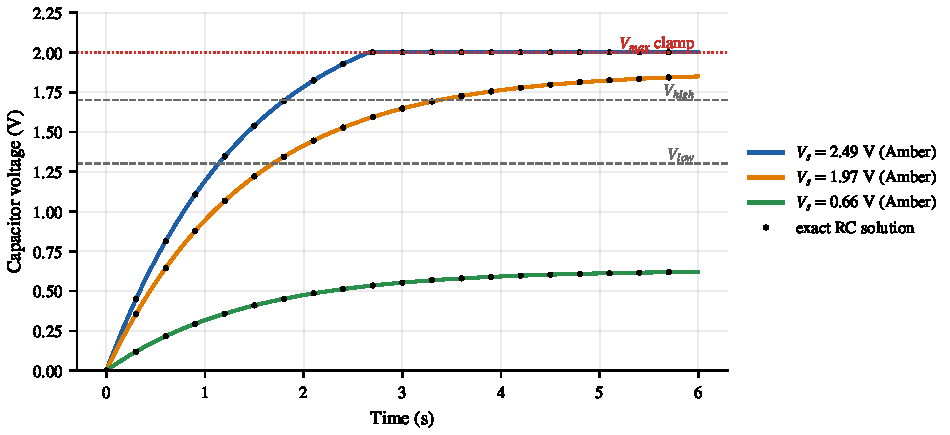
\includegraphics[width=0.9\linewidth]{fig_cap_charge}
\caption{Charging from empty for three source voltages. Lines: Amber's discrete update; dots: the exact solution Eq.~\eqref{eq:vsol} (they coincide). The top curve is clipped by $\Vmax=\SI{2}{V}$. The bottom curve ($\Vs=\SI{0.66}{V}$) saturates far below $\Vlow$ and never activates a node.}
\label{fig:capcharge}
\end{figure}

\section{Discretisation: how Amber steps the equation}
\label{sec:discretisation}

Amber advances the capacitor in steps of $\Delta t=\SI{1}{ms}$. Because
$\Delta t/\tau\approx7\times10^{-4}\ll1$, even a crude scheme is accurate;
Amber uses a hybrid of two methods per step. For the charge-only case:
\begin{equation}
 V_{k+1}=V_k\,\e^{-\Delta t/(\Rl C)}+\frac{\Delta t}{\Rs C}\big(\Vs-V_k\big).
\label{eq:chargestep}
\end{equation}
The leakage term is integrated \emph{exactly} (an exponential decay), the source
term by one \emph{explicit-Euler} step; this is an \emph{operator-splitting}
scheme with error $O(\Delta t)$ per unit time. Explicit Euler is stable here because $\Delta t/(\Rs C)\ll2$.

\begin{keyidea}[Verified: the charge-only step is accurate to $2\times10^{-4}$ V]
Starting from $\SI{1.0}{V}$ with $\Vs=\SI{2.5}{V}$ (unclamped), after $\SI{1}{s}$ Amber gives
$\SI{1.69536}{V}$; the exact solution Eq.~\eqref{eq:vsol} gives $\SI{1.69519}{V}$.
\end{keyidea}

\subsection{The four step types}

The \code{Capacitor} class implements four updates; the controller selects among them by sending a SimPy \emph{interrupt}
with a string cause (Chapter~\ref{ch:architecture}). Each ends with a clamp to $[0,\Vmax]$ ($\Vmax=\SI{2}{V}$, ``physical clamp / PMIC max'').
\begin{center}
\small
\renewcommand{\arraystretch}{1.3}
\begin{tabularx}{\linewidth}{@{}>{\ttfamily}p{3.8cm}X@{}}
\toprule
\normalfont\bfseries Cause (interrupt) & \normalfont\bfseries Update (per $\Delta t$)\\
\midrule
\codew{capacitor_charging} & Eq.~\eqref{eq:chargestep}: charge from $\Vs$ with leakage. Used while off or waiting for a slot.\\
\codew{capacitor_full} & Leakage only: $V\leftarrow V\,\e^{-\Delta t/(\Rl C)}$. Sent once, at activation.\\
\codew{capacitor_discharge} & Load only: $\Delta E=V I\Delta t$, $V\leftarrow\sqrt{V^2-2\Delta E/C}-V(1-\e^{-\Delta t/\Rl C})$. \emph{Not sent by the shipped controller.}\\
\codew{capacitor_charge_and_discharge} & Simultaneous: $I_c=\max\{(\Vs-V)/\Rs,0\}$; $E\leftarrow\max\{E+\Vs I_c\Delta t-VI_L\Delta t,\,0\}$; $V\leftarrow\sqrt{2E/C}\,\e^{-\Delta t/\Rl C}$. Used in every active state.\\
\bottomrule
\end{tabularx}
\end{center}

\paragraph{The capacitor is passive.}
The \code{Capacitor}'s own process merely \emph{waits}; its voltage changes
\emph{only when the controller interrupts it}. Because the controller issues exactly one interrupt per millisecond, one controller tick equals
one capacitor step. As we verified experimentally, SimPy schedules an interrupt with
\emph{urgent} priority, so the capacitor reacts within the \emph{same} millisecond, before ordinary events at that time. A capacitor created without a
controller would hold its voltage forever, with no leakage.

\subsection{Discharge}
Under a constant-current load $I_L$ the leakage-free solution of Eq.~\eqref{eq:ode} is
$V(t)=V_0-I_Lt/C$. Amber states this via \emph{energy}: the load draws power $VI_L$,
so in one step $\Delta E=VI_L\Delta t$ and $V'=\sqrt{V^2-2\Delta E/C}\approx V-I_L\Delta t/C$ for small steps---the same result. A $\SI{15}{ms}$, $\SI{5}{mA}$ transmission therefore
lowers a capacitor of $\SI{300}{\micro F}$ by
\[
 \Delta V=\frac{I_L\,T}{C}=\frac{5\times10^{-3}\cdot15\times10^{-3}}{300\times10^{-6}}=\SI{0.25}{V},
\]
which is exactly the step height of the sawtooth in Figure~\ref{fig:sawtooth} (we measured $1.5\to1.248$~V
for the load-only step, against $1.25$~V for ideal constant current).

\section{Thresholds, hysteresis and the energy window}
\label{sec:hysteresis}

A node cannot operate at an arbitrarily low voltage, and turning it on at the
\emph{same} voltage at which it turns off would cause \emph{chattering}: starting up draws current,
the voltage sags below the threshold, the node switches off, the voltage recovers, and so on. The remedy
is \emph{hysteresis}, familiar from the Schmitt trigger and from the under-voltage lock-out of
energy-harvesting power-management ICs: two thresholds.
\begin{itemize}
 \item \textbf{$\Vhigh$} (demo: $\SI{1.7}{V}$): the node switches \emph{on} when $V\ge\Vhigh$.
 \item \textbf{$\Vlow$} (demo: $\SI{1.3}{V}$): the node switches \emph{off} when $V\le\Vlow$.
\end{itemize}
\begin{figure}[t]
\centering
\begin{tikzpicture}[node distance=5.2cm]
 \node[st,draw=agrey,fill=lightgrey,minimum width=3.4cm] (off) {Charging (off)\\harvest only, no load};
 \node[st,draw=agreen,fill=lightgreen,minimum width=3.4cm,right=of off] (on) {Active\\duty cycle (load on)};
 \draw[->,thick] (off.north) to[bend left=35] node[lab,above,align=center]{$V\ge\Vhigh$\\and start-up delay over} (on.north);
 \draw[->,thick] (on.south) to[bend left=35] node[lab,below]{$V\le\Vlow$} (off.south);
\end{tikzpicture}
\caption{Hysteretic two-state behaviour of an energy-harvesting node. The $\SI{0.4}{V}$ gap between thresholds sets the size of the usable energy window.}
\label{fig:hyst}
\end{figure}
The energy available between the thresholds is
\begin{equation}
 \Delta E=\tfrac12C\big(\Vhigh^2-\Vlow^2\big)=\tfrac12(300\,\mu\mathrm{F})(1.7^2-1.3^2)=\SI{180}{\micro J}.
\end{equation}
The stored energy at $\SI{1.7}{V}$ is $\SI{433.5}{\micro J}$, of which only $41\%$ is usable;
the rest remains as the unusable floor $\tfrac12C\Vlow^2=\SI{253.5}{\micro J}$. A
larger $C$ gives a larger window (longer bursts, longer recharge); a wider gap does too.

\paragraph{How many packets fit in one window?}
We will see in Chapter~\ref{ch:controller} that one full node cycle (listen, sense, process, transmit)
consumes about $\SI{125}{\micro J}$, of which $90\%$ is the $\SI{15}{ms}$
transmission. The window of $\SI{180}{\micro J}$ would therefore hold only $\approx1.4$ cycles without
harvesting. The measured behaviour is a useful check on this arithmetic. In a $\SI{20}{s}$ run of the broadcast demo, Node~0 completed
$23$ charge cycles and sent $47$ packets, Node~1 sent $18$ in $9$ cycles and Node~2 sent $56$ in $27$ cycles:
\textbf{about two packets per saw-tooth tooth}. The first transmission of a tooth runs to completion
($\SI{15}{ms}$); the second is typically \emph{cut short}, because $V$ reaches $\Vlow$ after only
$9$--$\SI{11}{ms}$ (visible in Figure~\ref{fig:fsmzoom}). We return to this in Chapter~\ref{ch:controller}.

\begin{keyidea}[Design rule: the window must cover an atomic burst]
If an operation cannot be interrupted (a radio transmission, a flash write), the energy window
$\tfrac12C(\Vhigh^2-\Vlow^2)$ minus what the node has already spent must exceed the energy of that atomic burst, or
the node will die in the middle of it. Amber does \emph{not} enforce this: the node simply powers
down whenever $V\le\Vlow$, wherever it happens to be in its state machine.
\end{keyidea}

\subsection{The duty-cycle theorem}

Let the net charging power into the capacitor be $P_{\mathrm{in}}$ while the node is off, and let the node draw
$P_{\mathrm{act}}>P_{\mathrm{in}}$ while active (approximating both as constant). One cycle consists of
recharging by $\Delta E$ and then spending it:
\[
 T_c=\frac{\Delta E}{P_{\mathrm{in}}},\qquad T_a=\frac{\Delta E}{P_{\mathrm{act}}-P_{\mathrm{in}}}.
\]
The fraction of time the node is active is
\begin{equation}
 D=\frac{T_a}{T_a+T_c}=\frac{\dfrac1{P_{\mathrm{act}}-P_{\mathrm{in}}}}{\dfrac1{P_{\mathrm{act}}-P_{\mathrm{in}}}+\dfrac1{P_{\mathrm{in}}}}
 =\frac{P_{\mathrm{in}}}{P_{\mathrm{act}}}.
\label{eq:duty}
\end{equation}
\begin{keyidea}[Duty-cycle theorem]
The long-run fraction of time an intermittently powered node is active equals the
ratio of harvested power to active-mode power, \emph{independent of the energy window}
$\Delta E$. The window ($C$, $\Vhigh$, $\Vlow$) determines only the \emph{granularity}: how long each active
burst and each recharge pause lasts, not how much activity there is on average.
\end{keyidea}
Energy neutrality ($\overline{P}_{\mathrm{consumed}}=\overline{P}_{\mathrm{in}}$) is Eq.~\eqref{eq:duty} in disguise.
For Node~0 at $V\approx\SI{1.5}{V}$ the capacitor receives about $\SI{0.30}{mW}$ (Section~\ref{sec:amberharvest}); if the node
transmitted continuously ($\SI{7.5}{mW}$ at $\SI{1.5}{V}$) it could be active only $D\approx4\%$ of the time.

\subsection{What the node forgets}
In the language of \emph{intermittent computing} \citep{lucia2017} a power failure erases volatile state. Amber's controller resets its
state machine to \emph{listening} at each reactivation, but \emph{keeps} the last processed sensor value
and the node's protocol state (for example, whether it is registered). That models non-volatile memory for
registration; a design that loses registration at every outage would behave differently.

\begin{reality}[The active-mode step credits source energy, not delivered energy]
The charge-only step, Eq.~\eqref{eq:chargestep}, is the exact RC behaviour: the power delivered into the capacitor is $P_h\,x(1-x)$ (Figure~\ref{fig:powertransfer}).
The \emph{charge-and-discharge} step used in every active state computes the energy gained as $\Vs\,I_c\,\Delta t$, where
$I_c=(\Vs-V)/\Rs$. That is the energy \emph{drawn from the source},
which includes the heat dissipated in $\Rs$; the energy actually stored is $V\,I_c\,\Delta t$. The simulator therefore over-credits harvesting by the factor $\Vs/V$ whenever a node is active.
\begin{figure}[H]
\centering
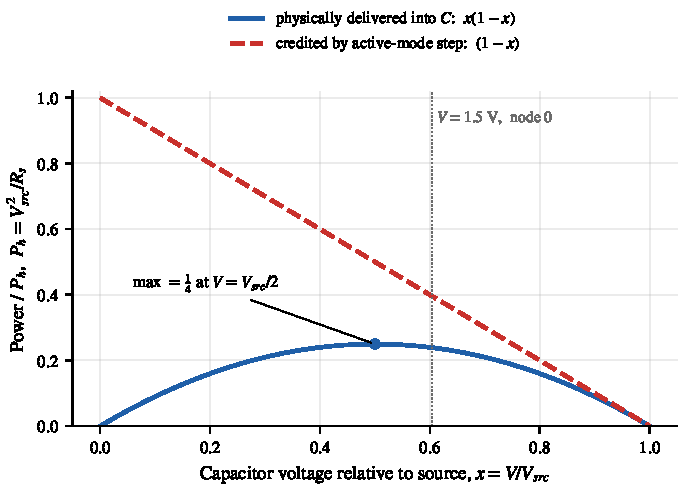
\includegraphics[width=0.55\linewidth]{fig_power_transfer}
\caption{Power delivered into $C$ (solid) versus the power credited by the active-mode step (dashed), both relative to $P_h=\Vs^2/\Rs$.}
\label{fig:powertransfer}
\end{figure}
We measured the effect directly. With zero load the two steps should agree; instead, starting from $\SI{1}{V}$ with $\Vs=\SI{2.5}{V}$, after $\SI{1}{s}$ the charge-only step reaches $\SI{1.695}{V}$ (exact: $\SI{1.695}{V}$) and the charge-and-discharge step $\SI{1.948}{V}$ (Figure~\ref{fig:energyaccounting}).
\begin{figure}[H]
\centering
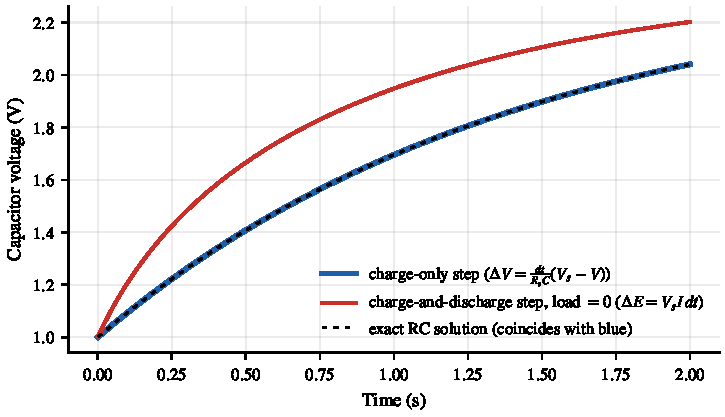
\includegraphics[width=0.78\linewidth]{fig_energy_accounting}
\caption{Zero-load charging from $\SI{1}{V}$: the charge-only step coincides with the exact RC solution; the charge-and-discharge step charges faster.}
\label{fig:energyaccounting}
\end{figure}
For the shipped demos the practical impact is small because the load dominates the active-state energy budget. Re-running the broadcast scenario ten times with a patched step that credits $V I_c\Delta t$ reduced the mean number of packets sent in $\SI{20}{s}$ from $124.4$ to $121.0$ ($\approx-2.7\%$). The effect would be larger for light loads or long active phases. Keep it in mind when interpreting duty-cycle numbers.
\end{reality}

\section{Chapter summary}
\begin{itemize}
 \item $C\,\dot V=(\Vs-V)/\Rs-V/\Rl-I_L$ gives $V(t)=V_\infty+(V_0-V_\infty)\e^{-t/\tau}$; $V_\infty=(\Vs-I_L\Rs)\Rl/(\Rl+\Rs)$; $\tau=(\Rs\parallel\Rl)C$.
 \item A node can sustain a current $I_{\max}=(\Vs-V)/\Rs-V/\Rl$; nodes whose typical load exceeds it must duty-cycle or starve.
 \item Amber advances the capacitor with a 1~ms hybrid step (exact leakage, Euler source). The charge-only step matches the exact solution to $2\times10^{-4}$~V.
 \item Hysteresis ($\Vhigh>\Vlow$) avoids chattering; $\Delta E=\tfrac12C(\Vhigh^2-\Vlow^2)=\SI{180}{\micro J}$ in the demos.
 \item Duty-cycle theorem: $D=P_{\mathrm{in}}/P_{\mathrm{act}}$.
 \item The active-mode step over-credits harvest by $\Vs/V$; $\approx3\%$ effect on demo packet counts.
\end{itemize}

\begin{codemap}
\small
\begin{tabularx}{\linewidth}{@{}>{\ttfamily}p{5.0cm}X@{}}
\toprule
\normalfont\bfseries Concept & \normalfont\bfseries Code (\file{amber/capacitor.py}, \file{controller.py})\\
\midrule
$R_s,R_l,C,\Delta t$ & \codew{CapacitorParams}\\
Eq.~\eqref{eq:chargestep} & \codew{Capacitor.capacitor_charging}\\
Leakage only & \codew{Capacitor.capacitor_selfdischarge}\\
Load only & \codew{Capacitor.load_discharging}\\
Charge + discharge & \codew{Capacitor.charge_and_discharge}\\
Clamp $\Vmax$ & \code{voltage_max}\\
Thresholds & \codew{VoltageThresholdsV(high, low)}\\
Who steps the capacitor & \codew{Controller.run}, via \codew{action.interrupt(cause)}\\
\bottomrule
\end{tabularx}
\end{codemap}

\section*{Exercises}
\begin{exercise}
For $\Rs=\SI{5}{k\ohm}$, $\Rl=\SI{100}{k\ohm}$, $C=\SI{200}{\micro F}$ (the SIC demo): compute $\tau$, and the time to charge from $0$ to $\SI{1.7}{V}$ with $\Vs=\SI{2.486}{V}$.
\end{exercise}
\begin{exercise}
A node draws a constant $\SI{300}{\micro A}$ while active. For what source voltages $\Vs$ is it energy-starved at $\Vlow=\SI{1.3}{V}$ (use $V_\infty<\Vlow$ with the load included)?
\end{exercise}
\begin{exercise}
Compute $\Delta E$ for $C=\SI{200}{\micro F}$, $\Vhigh=\SI{1.7}{V}$, $\Vlow=\SI{1.3}{V}$. By what factor must $C$ change to double the usable window? What if instead $\Vlow$ were lowered to $\SI{1.1}{V}$?
\end{exercise}
\begin{exercise}
Derive Eq.~\eqref{eq:tth} and verify the entry $t=\SI{3.37}{s}$ for Node~1 ($\Vs=\SI{1.971}{V}$).
\end{exercise}
\begin{exercise}
A node harvests $P_{\mathrm{in}}=\SI{200}{\micro W}$ into its capacitor and, while active, draws $\SI{4}{mW}$. What is its long-run duty cycle? Using the energy window $\Delta E=\SI{180}{\micro J}$, estimate $T_c$, $T_a$ and the number of active bursts per second.
\end{exercise}
\begin{exercise}
Show that the maximum of $V(\Vs-V)/\Rs$ over $V$ is $\Vs^2/(4\Rs)$, and use this to explain why the model never delivers more than $25\%$ of the nominal harvested power.
\end{exercise}
